\documentclass{hw}

\usepackage{pythontex}

\renewcommand\emph[1]{{\bf\color{BlueViolet}#1}}

\title{PHYS 2214 -- Prelim 1}

\begin{document}
\maketitle

\tableofcontents{}
\newpage{}

%%%%%%%%%%%%%%%%%%%%%%%%%%%%%%%%%%%%%%%%%%%%%%%%%%%%%%%%%%%%%%%%%%%%%%%%%%%%%%%%
\section{Disclaimer}
The math and reasoning presented below is scribed from the lecture notes. I
guarantee neither its correctness nor its sanity. If you notice a scribing
error or an inconsistency with the notes, please bring it to my attention.

Some math will be hand waved. Bear with me.

%%%%%%%%%%%%%%%%%%%%%%%%%%%%%%%%%%%%%%%%%%%%%%%%%%%%%%%%%%%%%%%%%%%%%%%%%%%%%%%%
\section{Oscillation}
A \emph{mechanical oscillation} is any repetitive motion. A \emph{free
oscillation} is oscillation with two properties:
\begin{enumerate}
  \item $\exists$ an $x_{eq}$ such that $F(x_{eq}) = 0$.
  \item When the object is displaced a small amount, the force restores the
    object to $x_{eq}$. This is a \emph{restoring force}. The equilibrium is
    \emph{stable}.
\end{enumerate}
Mathematically, we can summarize these properties for the two-dimensional case
as
\[\cbox{
  F(x_{eq}) = 0, \quad \left.\frac{dF}{dx}\right|_{x_{eq}} < 0
}\]

%%%%%%%%%%%%%%%%%%%%%%%%%%%%%%%%%%%%%%%%%%%%%%%%%%%%%%%%%%%%%%%%%%%%%%%%%%%%%%%%
\section{Simple Harmonic Motion (SHM)}
\emph{SHM} is a special type of oscillation where position is a sinusoidal
function of time.
\begin{gather*}
  \cbox{x(t) = A\cos(\omega t + \phi)} \\
  \cbox{v(t) = x'(t) = -A \omega \sin(\omega t + \phi)} \\
  \cbox{a(t) = x''(t) = -A \omega^2 \cos(\omega t + \phi) = -\omega^2 x(t)} 
\end{gather*}

\begin{claim}
If an object is acted upon by a \emph{linear restoring force}, $F \propto -x$,
then it will undergo SHM.
\begin{proof}
Assume the constant of proportionality for the linear restoring force is $k$.
From Newton's laws the properties of SHM, we have:
\begin{align*}
  F &= ma \\
    &= -m \omega^2 x \\
    &= -k x \\
  \omega &= \sqrt{\frac{k}{m}}
\end{align*}
\end{proof}
\end{claim}

$\omega$, or $\omega_0$, is the \emph{natural frequency} of oscillation. It is
the frequency at which an object oscillates if displaced.

%%%%%%%%%%%%%%%%%%%%%%%%%%%%%%%%%%%%%%%%%%%%%%%%%%%%%%%%%%%%%%%%%%%%%%%%%%%%%%%%
\section{Damped Oscillations}
A \emph{damping force} is a force that acts opposite of motion. Consider a
damping force that varies linearly with velocity. 
\begin{gather*}
  F = ma = -kx -bv \\
  mx'' + bx' + kx = 0
\end{gather*}
Ah, the good old fashioned oscillator equation. Let's use complex numbers to
solve this familiar beast. Let $z(t) = Ae^{\alpha t}$ where $\alpha$ is some
complex number. We'll also use plenty of hand waving.
\begin{gather*}
  mz'' + bz' + kz = 0 \\
  (m\alpha^2 + b\alpha + k)z = 0 \\
  \cbox{\alpha = \frac{-b \pm \sqrt{b^2 - 4mk}}{2m}}
\end{gather*}
We can now do a case analysis on $b$, $m$, and $k$. Also let $x = \Re({z})$.
Final equations for $x(t)$ will be highlighted a distinct color.

\subsection{Very Underdamped}
Assume $\cbox{b^2 \ll 4mk}$. If $b^2$ is much much smaller than $4mk$, then we
can ignore $b^2$.
\begin{align*}
  \alpha &= \frac{-b \pm \sqrt{b^2 - 4mk}}{2m} \\
         &\approx \frac{-b \pm \sqrt{-4mk}}{2m} \\
         &= \frac{-b}{2m} \pm \frac{\sqrt{-4mk}}{2m} \\
         &= \frac{-b}{2m} \pm \frac{\sqrt{-4mk}}{\sqrt{4m^2}} \\
         &= \frac{-b}{2m} \pm \sqrt{\frac{-4mk}{4m^2}} \\
         &= \frac{-b}{2m} \pm \sqrt{\frac{-k}{m}} \\
         &= \frac{-b}{2m} \pm i\sqrt{\frac{k}{m}} 
\end{align*}

Substituting $\alpha$ into $z$.
\begin{align*}
  z &= Ae^{\alpha t} \\
    &= Ae^{(\frac{-b}{2m} \pm i\sqrt{\frac{k}{m}})t} \\
    &= Ae^{\frac{-b}{2m}t} \pm e^{i\sqrt{\frac{k}{m}}t} \\
  x &= Ae^{\frac{-b}{2m}t} \cos\left(\sqrt{\frac{k}{m}}t\right) 
\end{align*}

After syntactic reduction,
\[\cbox[blue]{
  \tau_A = \frac{2m}{b}, \quad
  \omega_0 = \sqrt{\frac{k}{m}}, \quad
  x(t) = Ae^{-t/\tau_A} \cos(\omega_0 t)
}\]
$\tau_A$ is the \emph{amplitude decay time}. 

The very underdamped case is a decaying sinusoid.

\subsection{Very Overdamped}
Assume $\cbox{b^2 \gg 4mk}$. Now, we ignore the $4mk$ in the numerator.
\begin{align*}
  \alpha &= \frac{-b \pm \sqrt{b^2 - 4mk}}{2m} \\
         &\approx \frac{-b \pm \sqrt{b^2}}{2m} \\
         &= \frac{-2b}{2m} \\
         &= \frac{b}{m}
\end{align*}

Again substitute $\alpha$ into $z$.
\begin{align*}
  z &= Ae^{\alpha t} \\
    &= Ae^{\frac{b}{m} t} 
\end{align*}

This time, the syntactic reduction is a bit contrived but yields some nice
consistency.
\[\cbox[blue]{
  \tau_A = \frac{m}{b}, \quad x(t) = Ae^{-t/\tau_A}
}\]

Unlike in the very underdamped case, the object here does not undergo any
oscillation. It decays immediately and monotonically to equilibrium.

\subsection{Critically Damped}
Assume $\cbox{b^2 = 4mk}$. As I pull the wool over your eyes and wave my hands
around, it becomes clear from the divine inspiration of Healey himself that
$\alpha$ has a double root. It follows with the utmost triviality:
\[\cbox[blue]{
  \tau_A = \frac{2m}{b}, \quad x(t) = (A + Bt)e^{-t/\tau_A}
}\]
As if arbitrated by a deity, the powers that be declare that $A$ and $B$ are
determined by initial conditions. What initial conditions? Only God knows now,
only God knows. Now, quick onto the next section!

\subsection{Energy in Damped Oscillators}
Total energy $E$, kinetic energy $K$, and potential energy $U$ can be related
as $E = K + U$. In an underdamped setting, energy oscillates between $K$ and
$U$. Recall that in an underdamped setting $x(t) = Ae^{-t/\tau_A} \cos(\omega_0
t)$ and consider the following.
\begin{align*}
  E &\approx U_{\text{max}} \\
    &\propto x_{\text{max}}^2 \\
    &\propto (e^{-t/\tau_A})^2 \\
    &= e^{2t/\tau_A} \\
    &=: e^{t/\tau_E}
\end{align*}

Tautologically,
\[\cbox{
  \tau_E = \frac{\tau_A}{2}
}\]

$\tau_E$ is the \emph{energy decay time}. 

%%%%%%%%%%%%%%%%%%%%%%%%%%%%%%%%%%%%%%%%%%%%%%%%%%%%%%%%%%%%%%%%%%%%%%%%%%%%%%%%
\section{Driven Oscillations}
Drive a damped oscillator with a sinusoidal force at frequency $\omega_D$. The
\emph{steady state response} of a linear system will be \emph{sinusoidal at the
drive frequency}, not at the natural frequency. We can characterize the
response with an amplitude $A(\omega_D)$ and phase $\phi(\omega_D)$, both
functions of $\omega_D$.

If we plot $A(\omega_D)$ against $\omega_D$, we'll find a \emph{response curve}
that resembles a Gaussian. The response curve has a maximum near $\omega_0$.
This maximum is called a \emph{resonance}.

Consider the set of frequencies that produce large amplitudes $S =
\setst{\omega_D}{A(\omega_D) \geq \frac{A_{max}(\omega_D)}{\sqrt{2}}}$. Define
the \emph{full width at half energy} $\cbox{\Delta \omega = \max(S) -
\min(S)}$. Similarly define the peakiness \emph{quality factor} $\cbox{Q =
\frac{\omega_r}{\Delta \omega}}$. An example frequency response curve is given
in Figure~\ref{fig:frequency-response}.

\begin{figure}[h]
  \centering
  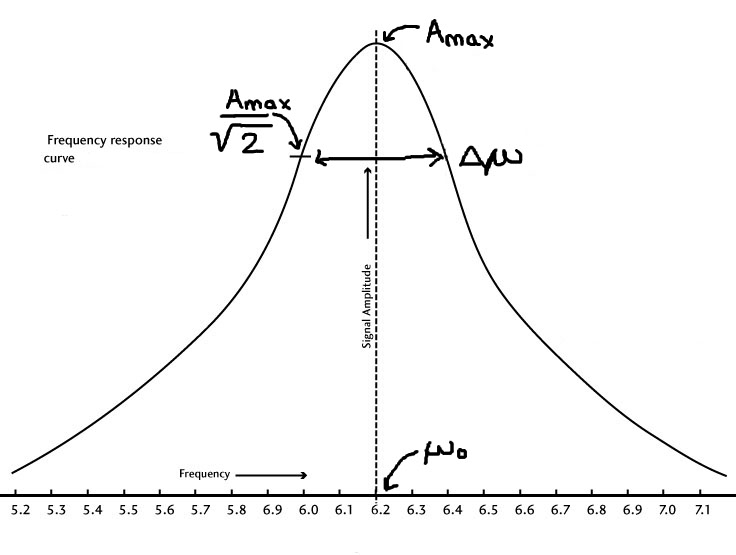
\includegraphics[width=0.75\textwidth]{img/frequency-response.jpg}
  \caption{%
    A frequency response curve. $\Delta \omega$ is a measure of the curve's
    width. $Q$ is a measure of the curve's perkiness.
  }
  \label{fig:frequency-response}
\end{figure}

Now, we'll dive into the math behind driven oscillations. Consider a driving
force $F_D(t) = F_0 \cos(\omega_D t)$. From Newton's laws, we get
\[
  mx'' + bx' + kx = F_D
\]
We'll use our favorite mathematical tool, hand waving, and make things a bit
more complex. Convert $F_D$ into $F_0 e^{i \omega_D t}$. Convert $x$ into
$Ae^{i\phi}e^{i \omega_D t}$. Now, we substitute these complex valued variables
into the differential equation.
\begin{align*}
  m(Ae^{i\phi}e^{i \omega_D t})'' + 
    b(Ae^{i\phi}e^{i \omega_D t})' + 
    k(Ae^{i\phi}e^{i \omega_D t}) &= F_0 e^{i \omega_D t} \\
  -\omega_D^2 m Ae^{i\phi}e^{i \omega_D t} + 
    i \omega_D b Ae^{i\phi}e^{i \omega_D t} + 
    k A e^{i\phi}e^{i \omega_D t} &= F_0 e^{i \omega_D t} \\
  (-\omega_D^2 m Ae^{i\phi} + 
    i \omega_D b Ae^{i\phi} + 
    k A e^{i\phi})e^{i \omega_D t} &= F_0 e^{i \omega_D t} \\
  -\omega_D^2 m Ae^{i\phi} + 
    i \omega_D b Ae^{i\phi} + 
    k A e^{i\phi} &= F_0 \\
    (-\omega_D^2 m  + i \omega_D b  + k) A e^{i \phi} &= F_0
\end{align*}
\begin{align*}
    A e^{i \phi} &= \frac{F_0}{-\omega_D^2 m  + i \omega_D b  + k} \\
                 &= \frac{F_0}{-\omega_D^2 m  + i \omega_D b  + k} 
                      \cdot \frac{1/m}{1/m} \\
                 &= \frac{F_0/m}{-\omega_D^2  + i \omega_D b/m  + k/m} \\
                 &= \frac{F_0/m}{k/m - \omega_D^2  + i \omega_D b/m} \\
                 &= \cbox{%
                      \frac{F_0/m}
                      {\omega_0^2 - \omega_D^2  + i \frac{2\omega_D}{\tau_A}}
                    } 
\end{align*}
$\cbox{\omega_0 = \sqrt{k/m}}$ and $\cbox{\tau_A = 2m/b}$.

Again, we can now do a case analysis on $\omega_0$ and $\omega_D$. Final
solutions for $x(t)$ will be accented in a similar, distinct color. All
solutions will have the form $\cbox{A \cos(\omega_D t + \phi)}$. Why, you ask?
Once upon a time, we and God knew. Now, only God knows.

\subsection{Low Frequencies}
Assume $\cbox{\omega_D \ll \omega_0}$. That is, we are driving at very low
frequencies compared to the resonance frequency. Because $\omega_D$ is so
small, we can neglect those terms and recompute $Ae^{i\phi}$.
\begin{align*}
  Ae^{i\phi} &= \frac{F_0/m}{\omega_0^2 - \omega_D^2  + i \frac{2\omega_D}{\tau_A}} \\
             &\approx \frac{F_0/m}{\omega_0^2} \\
             &\approx \frac{F_0}{\omega_0^2 m} \\
             &\approx \frac{F_0}{(\sqrt{k/m})^2 m} \\
             &\approx \frac{F_0}{\frac{k}{m} m} \\
             &\approx \frac{F_0}{k} 
\end{align*}

Substituting into our God equation above,
\[\cbox[green]{
  A = \frac{F_0}{k}, \quad \phi = 0, \quad x(t) = \frac{F_0}{k}\cos(\omega_D t)
}\]

Notice that at low frequencies, the response is determined completely by the
spring constant. Inertia and damping are both negligible.

\subsection{High Frequencies}
Assume $\cbox{\omega_D \gg \omega_0}$. That is, we are driving at very high
frequencies compared to the resonance frequency. Since $\omega_D$ is much
larger that $\omega_0$, we can ignore the $\omega_0$ in the equation for $Ae^{i
\phi}$. Also, $\omega_D^2$ dominates $\omega_D$, so we can ignore those terms
as well.
\begin{align*}
  Ae^{i\phi} &= \frac{F_0/m}{\omega_0^2 - \omega_D^2  + i \frac{2\omega_D}{\tau_A}} \\
             &= \frac{F_0/m}{-\omega_D^2} \\
             &= -\frac{F_0}{m\omega_D^2} \\
             &= \frac{F_0}{m\omega_D^2} e^{-i\pi} \tag*{$-1 = e^{-i\pi}$}
\end{align*}

\[\cbox[green]{
    A = \frac{F_0}{m\omega_D^2}, \quad 
    \phi = -\pi, \quad 
    x(t) = \frac{F_0}{m\omega_D^2}\cos(\omega_D t - \pi)
}\]

Notice that at high frequencies, the response is determined completely by the
inertia of the system. Damping and spring constants are negligible.

\subsection{Resonance}
Assume $\cbox{\omega_D = \omega_0}$. Now, $\omega_0^2 - \omega_D^2$ term in the
denominator of our $Ae^{i\pi}$ equation is 0.
\begin{align*}
  Ae^{i\phi} &= \frac{F_0/m}{\omega_0^2 - \omega_D^2  + i \frac{2\omega_D}{\tau_A}} \\
             &= \frac{F_0/m}{i \frac{2\omega_D}{\tau_A}} \\
             &= \frac{F_0}{i \frac{2 m \omega_D}{\tau_A}} \\
             &= -i\frac{F_0}{\frac{2 m \omega_D}{\tau_A}} \\
             &= -i\frac{F_0 \tau_A}{2 m \omega_D} \\
             &= -i\frac{F_0 \frac{2m}{b}}{2 m \omega_D} \\
             &= -i\frac{F_0}{b \omega_D} 
\end{align*}

\[\cbox[green]{
  A = \frac{F_0}{b \omega_D}, 
  \quad \phi = -\frac{\pi}{2},
  \quad \frac{F_0}{b \omega_0} \cos\left( \omega_0 t - \frac{\pi}{2} \right)
}\]

Notice that at resonance, the velocity is determined completely by the damping.
The inertia and sprint constant are negligible.

\subsection{Full Width and Quality Factor}
$\omega_r$ is not always at $\omega_0$. The lighter the damping, the more true
that this becomes. In a heavier damped system, the response may not even have a
resonance. After looking to the heavens, we also find
\[\cbox{
  \Delta \omega = \frac{2}{\tau_A} = \frac{1}{\tau_E}
}\]
and
\[\cbox{
  Q = \frac{\omega_0}{\Delta \omega} 
    = \omega_0 \tau_E 
    = \frac{1}{2} \omega_0 \tau_A 
    = \frac{\omega_0 m}{b}
}\]

$Q$ varies inversely with $b$.

\subsection{Power in Driven Oscillations}
Recall instantaneous power $P(t) = F(t)v(t)$. We can average instantaneous
power over a single cycle.
\[\cbox{
  P = \frac{1}{T} \int_{t_0}^{t_0 + T} P(t) dt
    = \frac{1}{T} \int_{t_0}^{t_0 + T} F(t)v(t) dt
}\]

Power is minimized at very low and very high frequencies. It is maximized at
resonance. This corresponds to velocity being out of phase and in phase with
the driving force respectively. We can also relate the gain of the response
curve to $Q$. In fact, they are equal.
\[\cbox{
  \text{gain} = \left| \frac{A(\omega_0)}{A(\omega_D \ll \omega_0)} \right| = Q
}\]

%%%%%%%%%%%%%%%%%%%%%%%%%%%%%%%%%%%%%%%%%%%%%%%%%%%%%%%%%%%%%%%%%%%%%%%%%%%%%%%%
\section{Traveling Waves}
A \emph{traveling wave} is defined by its properties:
\begin{itemize}
  \item A \emph{disturbance} propagates through a medium. Note that the medium
    itself is not propagating.
  \item The velocity is determined by the medium
\end{itemize}
Waves in which the medium disturbance is perpendicular to the wave velocity are
\emph{transverse waves}. Waves in which medium displacements are parallel to
wave velocity are \emph{longitudinal waves}.

%%%%%%%%%%%%%%%%%%%%%%%%%%%%%%%%%%%%%%%%%%%%%%%%%%%%%%%%%%%%%%%%%%%%%%%%%%%%%%%%
\section{Ideal Wave Motion}
An ideal wave travels at \emph{constant velocity} and with \emph{unchanging
shape}. In order for a medium to realize ideal motion:
\begin{itemize}
  \item The medium must be \emph{nondispersive}. All waves on a nondispersive
    medium have the same velocity, regardless of wavelength or amplitude. 
  \item The medium is \emph{linear}
  \item The wave \emph{must not be damped or amplified} as it travels.
\end{itemize}

%%%%%%%%%%%%%%%%%%%%%%%%%%%%%%%%%%%%%%%%%%%%%%%%%%%%%%%%%%%%%%%%%%%%%%%%%%%%%%%%
\section{Mathematical Description of an Ideal Transverse Traveling Wave}
The height of an ideal traveling wave is a function of both position along the
medium $x$ and time $t$. We can express the height as $y(x,t)$. By the
properties of a ideal wave motion, it follows that $y$ must be a function of $x
- vt$.
\[\cbox{
  y(x, t) = f(x \mp vt), \quad v > 0
}\]

From the definition of $f$ and with the help of partial derivatives, we can
derive two equations. The \emph{pulse equation}
\[\cbox{
  \frac{\partial y}{\partial t} = \mp v \frac{\partial y}{\partial x}
}\]
and the \emph{wave equation}
\[\cbox{ 
  \frac{\partial^2 y}{\partial t^2} = v^2 \frac{\partial^2 y}{\partial x^2}
}\]

%%%%%%%%%%%%%%%%%%%%%%%%%%%%%%%%%%%%%%%%%%%%%%%%%%%%%%%%%%%%%%%%%%%%%%%%%%%%%%%%
\section{Harmonic Traveling Waves}
A \emph{harmonic traveling wave} is a traveling wave with a sinusoidal
displacement. A harmonic traveling wave can be described mathematically as
$f(u) = A\cos(ku + \phi)$ where $u = x \mp vt$.
\[\cbox{
  y(x,t) = A\cos(k(x \mp vt) + \phi) = A\cos(kx \mp \omega t + \phi)
}\]
\[\cbox{
  k = \frac{2\pi}{\lambda}, \quad 
  \omega = 2 \pi f, \quad
  v = \frac{\omega}{k} = \frac{\lambda}{T} = f \lambda
}\]

$k$ is the \emph{wavenumber} and the is the parallel of frequency in the $x$
domain. $\lambda$ is the \emph{wavelength} of the wave.

We can commute our equation to the form
\[
  y(x,t) = A\cos(\mp \omega t + (kx + \phi))
\]
This makes it more clear that at a given fixed $x$, the medium undergoes
vertical simple harmonic motion. Also, $\forall x.\, \forall x'.\, A(x) =
A(x'), T(x) = T(x')$. In words, the amplitude and period of these vertical
simple harmonic motions are all equal. They differ only in their phase.

%%%%%%%%%%%%%%%%%%%%%%%%%%%%%%%%%%%%%%%%%%%%%%%%%%%%%%%%%%%%%%%%%%%%%%%%%%%%%%%%
\section{Waves on a String}
To simplify our analysis we make the following assumptions.
\begin{itemize}
  \item Displacements are purely transverse.
  \item The only force present is tension.
  \item Tension is constant throughout the string.
  \item Transverse displacements are small.
\end{itemize}

\begin{claim}
The horizontal forces on a small segment of wire sum to 0.
\begin{proof}
\begin{align*}
  \sum F_x &= \tau_{\text{right}} - \tau_{\text{left}} \\
           &= \tau\left[\cos(\theta(x + \Delta x, t)) - \cos(\theta(x, t)) \right] \\
           &\approx \tau (1 - 1) \\
           &= 0
\end{align*}
\end{proof}
\end{claim}

\begin{claim}
\[\cbox{
  \frac{\partial^2 y}{\partial t^2} = \frac{\tau}{\mu} \frac{\partial^2 y}{\partial x^2}
}\]
\begin{proof}
Recall a corollary the small angle approximation $\theta \approx 0 \implies
\frac{dy}{dx} \approx \tan(\theta)$. Also note that we will substitute $\sum F$
for $ma$ as per Newton's laws. 
\begin{align*}
  \sum F_y &= \tau\left[\sin(\theta(x + \Delta x, t)) - \sin(\theta(x, t)) \right] \\
           &\approx \tau \left[ y'(x + \Delta x, t) - y'(x, t) \right] \\
  ma       &= \tau \left[ y'(x + \Delta x, t) - y'(x, t) \right] \\
  a        &= \frac{\tau}{\mu} \frac{\left[ y'(x + \Delta x, t) - y'(x, t) \right]}
                {\Delta x} \\
  a        &= \frac{\tau}{\mu} y'' \\
  \frac{\partial^2 y}{\partial t^2} &= \frac{\tau}{\mu} \frac{\partial^2 y}{\partial x^2}
\end{align*}
\end{proof}
\end{claim}

A proof by pattern matching will show the following corollary holds.
\[
  \cbox{v = \sqrt{\frac{\tau}{\mu}}}
\]

%%%%%%%%%%%%%%%%%%%%%%%%%%%%%%%%%%%%%%%%%%%%%%%%%%%%%%%%%%%%%%%%%%%%%%%%%%%%%%%%
\section{Sound Waves} 
In fluids, waves are purely longitudinal. We can described these longitudinal
waves with two properties:
\begin{itemize}
  \item $s(x,t)$ is the displacement along the axis of displacement.
  \item $\Delta p(x,t) = p(x,t) - p_0$ is the variation in pressure.
\end{itemize}

First, we'd like to know the relationship between $\Delta p$ and $s$. To find
the relationship, we first define the \emph{bulk modulus} $B$ which is the
analog of a spring constant.
\[\cbox{
  \Delta p = \frac{\Delta F}{A} = -B \frac{\Delta V}{V}
}\]

\begin{lemma}
\[\cbox{
  \Delta p = -B \frac{\partial s}{\partial x}
}\]
\begin{proof}
Consider a column of fluid along the axis of a propagating sound wave. The
column of fluid has area $A$ and undisturbed length $\Delta x$. After it is
perturbed, the left end of the column is displaced to $x + s(x,t)$ and the left
end of the column is displaced to $x + \Delta x + s(x + \Delta x, t)$.

The change in volume $\Delta V$ is the change in displacement at $x$ and at $x
+ \Delta x$.
\[
  \Delta V = A[s(x + \Delta x, t) - s(x, t)]
\]

If we substitute this value into our equation for the bulk modulus, we find
\begin{align*}
  \Delta p &= -B \frac{\Delta V}{V} \\
           &= -B \frac{A[s(x + \Delta x, t) - s(x, t)]}{V} \\
           &= -B \frac{A[s(x + \Delta x, t) - s(x, t)]}{A \Delta x} \\
           &= -B \frac{[s(x + \Delta x, t) - s(x, t)]}{\Delta x} \\
           &\approx -B \frac{\partial s}{\partial x}
\end{align*}
\end{proof}
\end{lemma}

If we use Newton's laws, we can derive the wave equation for sound waves. I
elide the proof here, as my arms are tired from waving.
\[\cbox{
  \frac{\partial^2 s}{\partial t^2} = \frac{B}{\rho} \frac{\partial^2 s}{\partial x^2} 
}\]

The corollary of which is that 
\[\cbox{
  v = \sqrt{\frac{B}{\rho}}
}\]

Comparing the wave equation of sound waves to that of waves on a string, we
notice that $v$ can be described as
\[
  \sqrt{\frac{\text{springiness}}{\text{massiness}}}
\]

%%%%%%%%%%%%%%%%%%%%%%%%%%%%%%%%%%%%%%%%%%%%%%%%%%%%%%%%%%%%%%%%%%%%%%%%%%%%%%%%
\section{Standing Waves}
Compare harmonic traveling waves with harmonic standing waves. First, harmonic
traveling waves.
\begin{itemize}
  \item Travel at a constant speed
  \item Reflected at boundaries
  \item $\forall x.\, y(x, t)$ is harmonic
  \item $\forall x.\, \forall x'.\, A(x) = A(x')$
  \item The phase of vertical harmonic motion varies linearly with $x$
\end{itemize}
Now, standing waves.
\begin{itemize}
  \item $\forall x.\, y(x, t)$ is harmonic
  \item The amplitude of the harmonic motion varies sinusoidally with $x$
  \item $\forall x.\, \forall x'.\, \phi(x) = \phi(x')$
\end{itemize}

A \emph{standing wave} forms as the superposition of multiple travelling waves.
Thus, we can describe a standing wave $y(x,t)$ as the sum of two travelling
waves $A_t\cos(kx - \omega t + \phi)$ and $A_t\cos(kx + \omega t + \phi)$.
Using a trigonometric identity, it follows
\[\cbox{
  y(x,t) = 2A_t \cos(kx + \phi)\cos(\omega t)
}\]

A few observations drawn from this equation.
\begin{itemize}
  \item $y$ is a product of functions of $x$ and $t$. The wave no longer
    travels.
  \item $\forall x.\, y(x,t)$ is harmonic at $\omega$.
  \item The amplitude varies sinusoidally with $x$.
\end{itemize}

%%%%%%%%%%%%%%%%%%%%%%%%%%%%%%%%%%%%%%%%%%%%%%%%%%%%%%%%%%%%%%%%%%%%%%%%%%%%%%%%
\section{Standing Waves on a String}
Standing waves are not produced at all frequencies. At what frequencies do
standing waves form and what determines $\omega$, $k$, and $\phi$? It is the
boundary conditions.

For a string with two fixed ends, we have
\begin{gather*}
  \forall t.\, y(0, t) = 0 = 2 A_t \cos(\phi) \\
  \forall t.\, y(L, t) = 0 = 2 A_t \cos(kL + \phi)
\end{gather*}

Solving for $\phi$ and then $k$, we find
\[\cbox{
  \phi = \pi/2, \quad
  k_n = \frac{n\pi}{L}, \quad
  \lambda_n = \frac{2L}{n}, \quad
  f_n = \frac{nv}{2L}, \quad
  n \in \set{1, 2, \ldots}
}\]

The set of $x$ where $A(x,t) = 0$ for all time are called \emph{nodes}. The set
of $x$ where amplitude is maximized are called \emph{antinodes}. The set of $x$
between nodes are called \emph{loops}. The lowest frequency mode is called the
\emph{fundamental frequency}. The other frequencies are \emph{harmonics}.

%%%%%%%%%%%%%%%%%%%%%%%%%%%%%%%%%%%%%%%%%%%%%%%%%%%%%%%%%%%%%%%%%%%%%%%%%%%%%%%%
\section{Standing Sound Waves in Pipes}
As for harmonic waves on a string, we can write
\[
  \Delta p(x, t) = A_s \cos(kx + \phi) \cos(\omega t)
\]

\subsection{Pipe with Two Open Ends}
At an open end, $\Delta p = 0$. Just as with waves on a string,
\[\cbox{
  k_n = \frac{n\pi}{L}, \quad
  \lambda_n = \frac{2L}{n}, \quad
  f_n = \frac{nv}{2L}, \quad
  n \in \set{1, 2, \ldots}
}\]

\subsection{Pipe with One Closed End}
At the closed end, $s$ is a node which implies that $\Delta p$ is an antinode.
\[\cbox{
  \lambda_n = \frac{4L}{n}, \quad
  f_n = \frac{nv}{4L}, \quad
  n \in \set{1, 3, 5, \ldots}
}\]

%%%%%%%%%%%%%%%%%%%%%%%%%%%%%%%%%%%%%%%%%%%%%%%%%%%%%%%%%%%%%%%%%%%%%%%%%%%%%%%%
\section{Standing Waves and Resonance}
We saw that when we drove an underdamped system near its natural frequency, it
experienced its maximum amplitude. Standing waves have a similar pattern. In
fact, \emph{standing waves are resonances of an extended system}. Generally, if
we create travelling waves at frequencies in which the waves construct, there
will be a standing wave. If we create travelling waves at other frequencies,
there could be a mess of waves. At certain frequencies, they will destruct.
Unlike with the driven underdamped system, the extended system here could have
multiple resonances. Though, not all resonances are pretty.

%%%%%%%%%%%%%%%%%%%%%%%%%%%%%%%%%%%%%%%%%%%%%%%%%%%%%%%%%%%%%%%%%%%%%%%%%%%%%%%%
\section{Wave Interaction with Boundaries}
We'll now examine how travelling waves interact with various boundaries.

\subsection{Fixed End}
\[\cbox{g(u) = -f(-u)}\]

\subsection{Free End}
\[\cbox{g(u) = f(-u)}\]

\subsection{Matched Termination}
Say we attached a massless slip ring to a dashpot. We could null any reflected
waves. To do so, the dashpot must have a damping coefficient:
\[\cbox{
  \gamma = \frac{\tau}{v}
}\]

\subsection{Conjoined Mediums}
\begin{gather*}
  \cbox{Z = \frac{\tau}{v} = \mu v} \\
  \cbox{g(u) = Rf(-u)} \\
  \cbox{R = \frac{Z_1 - Z_2}{Z_1 + Z_2}} \\
  \cbox{h(u) = Tf(u)} \\
  \cbox{T = \frac{2Z_1}{Z_1 + Z_2} = 1 + R} \\
  \cbox{W_2 = \frac{v_2}{v_1}W_1}
\end{gather*}
\end{document}
